\chapter{Results}
\label{chap:simulation_results}
In this chapter, we present results for the estimation of actuation configuration for using both simulation data and data from the real system. \\

Since the parameter space of the motor configuration is not very intuitive for error analysis,
we transform the parameter results (and its variance) to a more intuitive form such that we can compare them.
%One possibility would be to express the motor position in the Cartesian blimp frame $b$.
%But since the position of the motor on the hull has only two degrees of freedom, a representation in the three dimensional blimp frame is not that much more intuitive.
A good possibility is to express the actuation configuration in the tangential reference frames $t^k$ (see \cref{sub:coordinate_systems}).
As the radius $r$ is not estimated, the estimation error in
$ \mathbf{e}_{t^k}^z $-direction is marginal.
\\
The error of the actuator arrangement is expressed by an error distance $e_{pos}^k$ for each motor $k$, which is approximated by the euclidean norm in the x-y plane of the tangential frame,
and an error angle $e_{angle}$, which is the angle between x-axes of the 'true' and estimated motor coordinate systems $\mathbf{e}_{m^k}^x$ and $\mathbf{e}_{t^k}^x$.

\begin{figure}[hbtp]
\centering
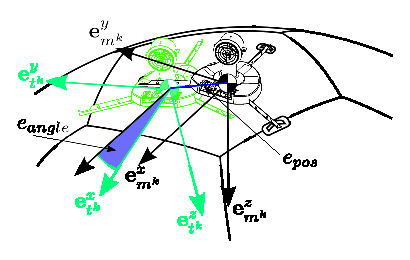
\includegraphics[width = 0.8\textwidth]{images/tangential_frame.eps}
\caption{The \textit{tangential frame} is the coordinate frame of the motor at its \textit{true} position. If the true position is not known, an estimate is used. In any case, its $\lbrace \mathbf{e}^x_{m^k} , \mathbf{e}^y_{m^k} \rbrace$ plane will be tangential to the spherical hull such that an error of the arrangement can be approximated by the euclidean norm in the tangential coordinate frame.}
\label{fig:tangential_frame}
\end{figure}

\section{Data used to generate Results}
\label{sec:bootstrapping_and_statistics}
To be able to generate meaningful results we recorded a long data set with Skye which contains about 850 seconds of undisturbed data samples.
To improve the accuracy of statistical results bootstrapping is applied to this large dataset.
Moving block bootstrapping is applied because the dataset consists of time series data. (??cite??)
The block stride is selected such that the dataset is divided in about 16 blocks.
According to margin of error (??cite??) calculations, the certainty that the actual standard deviation lies within 25\% of the standard deviation of the results from 16 blocks is 95\%. \\
Unless otherwise stated, the presented statistical results imply an 25\% error margin.

\section{Simulation}
For the following sections, a dataset has been generated from simulation of a blimp that is similar to Skye with a \unit[1.37]{m} radius.
The simulation includes aerodynamic drag as well as sensor noise.
The dataset is \unit[850]{s} long.
The same input vectors than in the real dataset have been applied.
%includes about the same number of input vectors than a real dataset from the blimp.

\subsection{Convergence}
\label{sec:sim_convergence}
In this section we are going to discuss the convergence properties of the batch optimisation.

\paragraph{Convergence w.r.t. dataset length} ~\\
In this thesis the datasets used for the batch optimisation have two concepts of length.
Individual input vectors are applied to the system for a fixed amount of time. \\
The first concept of length is thus measured in number of different input vectors, number of input vectors for short.
The second concept of length is the amount of data-samples are used during each of the different input vectors, number of samples per input vector for short. \\
The number of input vectors is the more important length measure as will be shown later.
It determines whether the parameters are observable at all. \\
The number of samples per input vector serves mainly to reduce the effect of the sensor noise on the results. \\
\Cref{fig:result_inputlength} shows the effects of different dataset lengths.
Below about 7 different input vectors no solution could be found. 
The number of samples per input vector reduces the error because noise from the sensors is reduced.

\begin{figure}[hbtp]
\centering
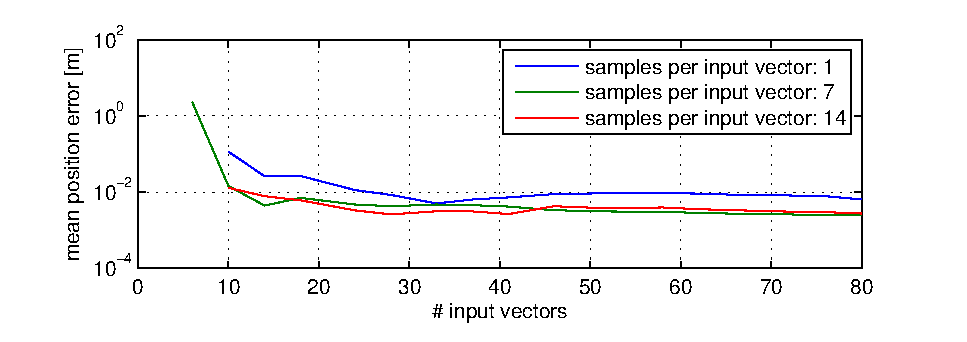
\includegraphics[width = \textwidth]{images/results/input_length_vs_position_error.eps}
\caption{Influence of the number of different input vectors on the mean position estimate error of the four AUs $e_{pos}$.
When using less than about 7 input vectors, no solution was found.
Number of samples per input vector decreases the error by reducing the influence of sensor noise}
\label{fig:result_inputlength}
\end{figure}

\paragraph{Convergence w.r.t. initial parameter estimate} ~\\
The impact of the initial parameter estimate on the convergence of the batch optimization has been tested.
In order to test convergence we implemented an algorithm which produces initial parameters from the true parameters.
It uses two metrics to distort the true parameters:
\begin{itemize}
\item Position deviation of each actuator on the hull surface
\item Rotation angle deviation of each actuator
\end{itemize}
The algorithm first rotates the actuator around its rotation axis by the given amount and then displaces it in a random direction on the hull surface by the requested amount. \\
For a grid of different position and angle deviations the failure rate was determined with ten samples each.
Figure~\ref{fig:result_sim_convergece_region} shows the result of this test.\\
It can be seen that an initial position offset of \textit{all} actuators in any random direction\footnote{
The simulated blimp has a hull radius of \unit[1.37]{m} and therefore the distance between two of the tetrahedrally arranged actuation units is \unit[2.62]{m}.}
is acceptable up to \unit[1]{m}.
Initial orientation offsets of the motors are acceptable up to \unit[120]{°}.
\\
The same observation can be made when using datasets from real measurements (compare \cref{fig:result_real_convergece_region}).
%Further results using real measurements are showed in the next section.


\begin{figure}[hbtp]
\centering
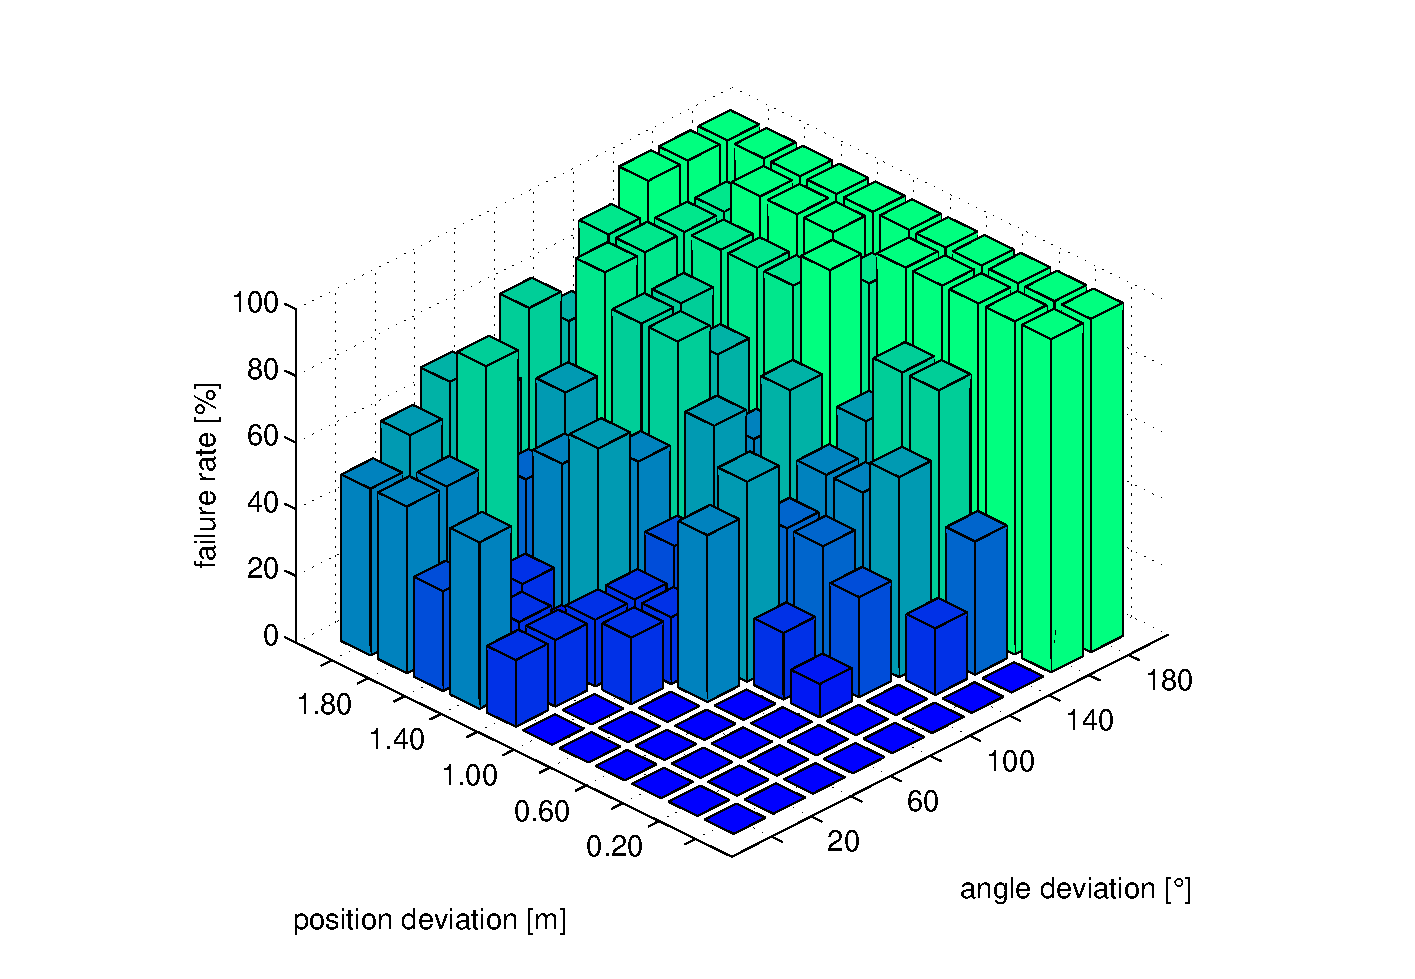
\includegraphics[width = \textwidth]{images/results/convergence_analysis_init_deviation_sim_bar.eps}
\caption{Failure rate using simulation data and different initial guess about actuation configuration.}
\label{fig:result_sim_convergece_region}
\end{figure}
\begin{figure}[hbtp]
\centering
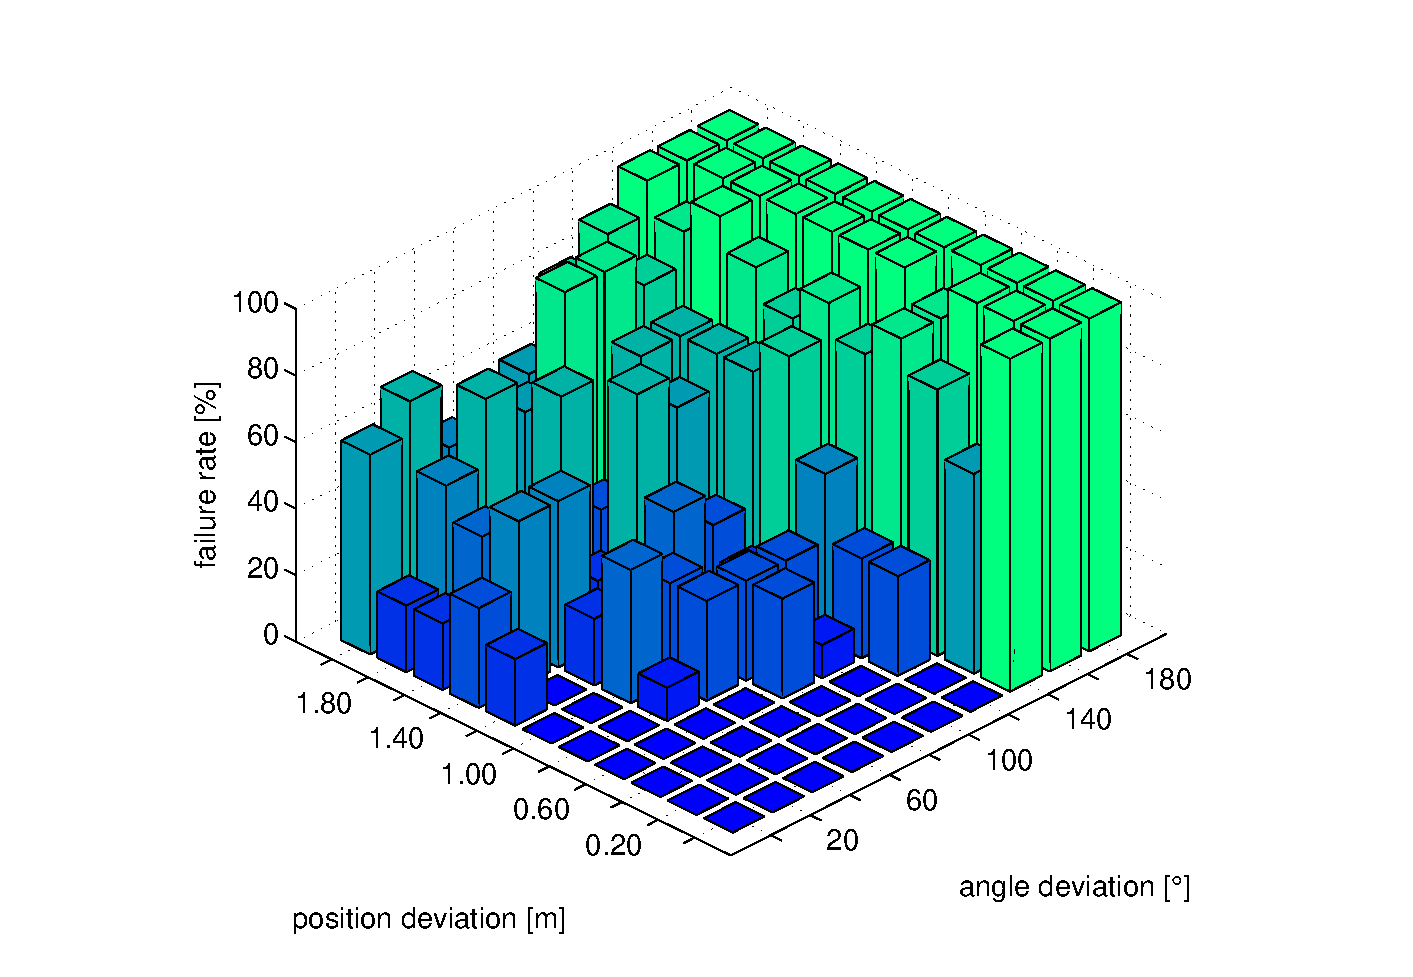
\includegraphics[width = \textwidth]{images/results/convergence_analysis_init_deviation_real_bar.eps}
\caption{Failure rate using experiment data and different initial guess about actuation configuration.}
\label{fig:result_real_convergece_region}
\end{figure}


\subsection{Estimation Confidence}
\paragraph{Methods} ~\\
In this thesis two methods have been used to determine  the confidence of the parameters.
The first method is outlined in section~\ref{sec:confidence_region} using the covariance matrices.
After the batch optimisation has found a set of optimal parameters, the covariance matrix is propagated through the coordinate transformations used to represent results.
The second method does not rely on any assumptions about covariance matrices and measures the parameter variance directly from multiple experimental results.
To get enough experimental results bootstrapping as described in section~\ref{sec:bootstrapping_and_statistics} is used to generate 16 different datasets.

\paragraph{Confidence from covariance matrix} ~\\
As introduced in \cref{sec:sim_convergence} there are two measures of dataset length which influence the result in different ways.
The same applies to the confidence calculated from the covariance matrix.
When using multiple samples per input vector the covariance matrix gets over-confident.
This means that the calculated variance is lower than the measured variance.
It is intuitively clear, that if we apply multiple times the same input vectors, we will not get more information about the actuation configuration.
The data samples are not independent.
When using just one sample per input vector, the calculated and measured variance match.

\paragraph{Confidence from multiple results} ~\\
As outline above the variance of the parameters has also been measured by evaluating multiple datasets generated from the same system and calculating the variance for each of the parameters.\\

In \cref{fig:result_95pc_confidence} the calculated variance is compared to the measured variance.
The variances are illustrated with circles that represent the region in which the parameters reside with 95\% certainty.
The size of the circles is determined with \cref{eq:variance_to_95pc}.

\begin{equation}
\label{eq:variance_to_95pc}
radius = 1.96 \cdot \sqrt{variance}
\end{equation}

\begin{figure}[hbtp]
\centering
%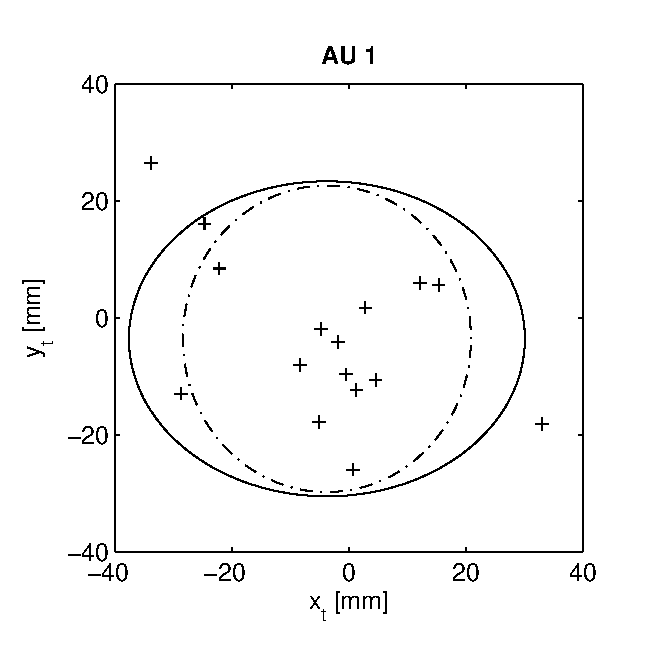
\includegraphics[width = 0.45\textwidth]{images/results/confidence_95_interval_AU1.eps}
%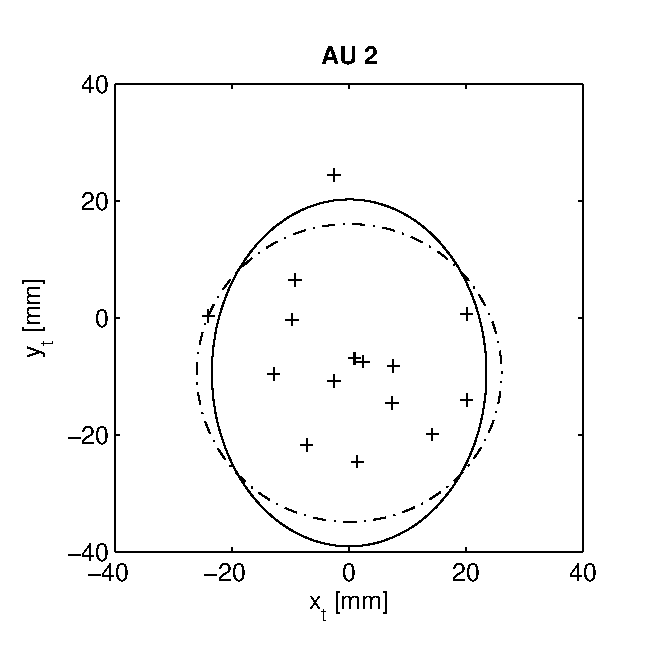
\includegraphics[width = 0.45\textwidth]{images/results/confidence_95_interval_AU2.eps} \\
%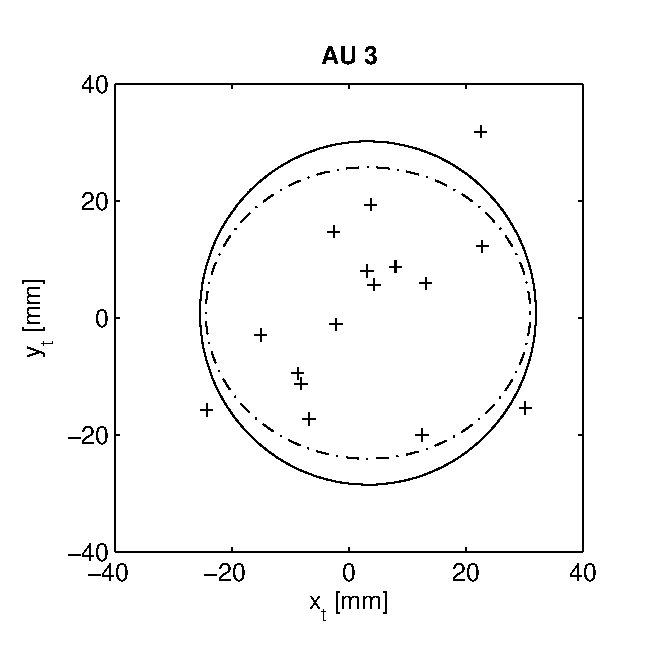
\includegraphics[width = 0.45\textwidth]{images/results/confidence_95_interval_AU3.eps}
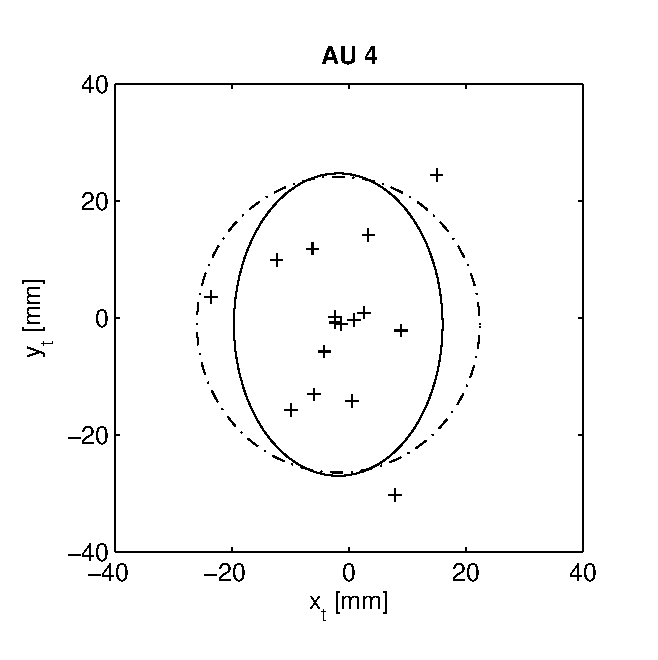
\includegraphics[width = 0.45\textwidth]{images/results/confidence_95_interval_AU4.eps}
\caption{Distribution of actuator position estimates. 16 datasets with 24 input vectors each and one sample per input vector.
$\mathbf{+}$ represent the results used to measure the variance.
\textbf{dashed}: 95\% confidence interval calculated from covariance matrix.
\textbf{solid}: 95\% confidence interval calculated from multiple results. }
\label{fig:result_95pc_confidence}
\end{figure}

\subsection{Estimation Performance}
\label{sub:est_perf}

To test the performance our optimization framework, we defined five test cases.
\begin{description}
\item[Default] A simulation of a blimp that is comparable to the real Skye system. All 21 parameters as listed in \cref{tab:params_updated} are estimated. This is the same test case as in the previous sections.
\item[1 AU] Same blimp as in default, but only one of the AUs is estimated (AU 4). The remaining AUs are not powered at all. 12 parameters estimated.
\item[5 AU] Different blimp with 5 AUs. Configuration for all AUs estimated. 24 parameters.
\item[No Drag] Same blimp as in default, but simulation without aerodynamic drag. This is used to see how much drag influences the result accuracy.
\item[COG] Same blimp as in default, but with large additional weight at AU4 position. COG to COB offset is 10cm and yields a moment in the same magnitude as the actuation moment. This is used to estimate the error introduced by large COG shifts.
\end{description}

For each of these test cases the RMS error for 4 different parameters has been calculated.
The samples for the RMS calculations are generated with the same method as described in section~\ref{sec:bootstrapping_and_statistics}.
The used parameters are:
\begin{enumerate}
\item Position error of AU 4 in the tangential frame
\item Angle error of AU 4 around the z axis of the tangential frame
\item Center of gravity error in the blimp frame
\item Tensor parameter vector error in percent
\end{enumerate}

Figure~\ref{fig:err_cmp_sim} shows the results of this analysis.

\begin{figure}[hbtp]
\centering
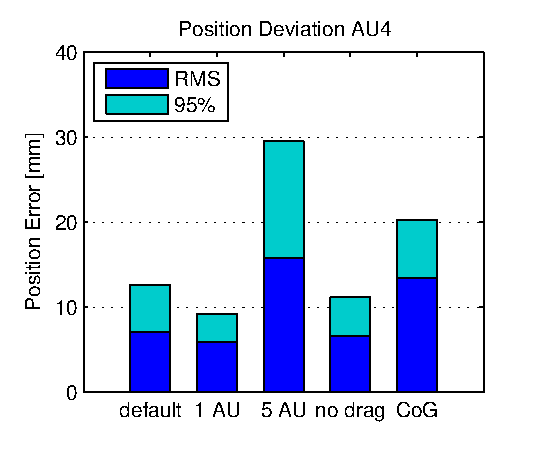
\includegraphics[scale=.72]{images/results/err_cmp_sim_pos.eps}
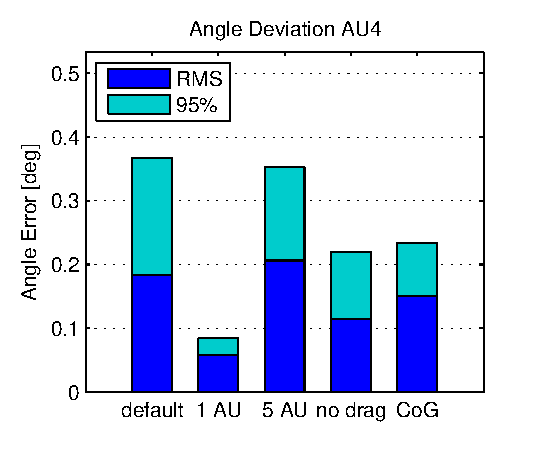
\includegraphics[scale=.72]{images/results/err_cmp_sim_angle.eps}
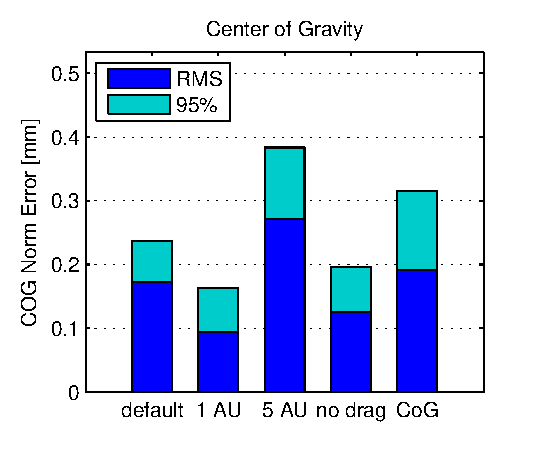
\includegraphics[scale=.72]{images/results/err_cmp_sim_cog.eps}
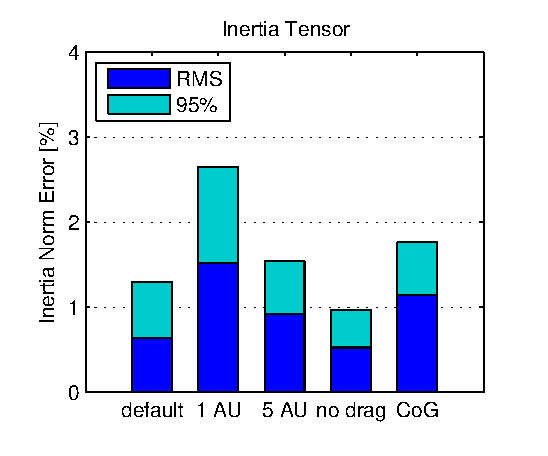
\includegraphics[scale=.72]{images/results/err_cmp_sim_tensor.eps}
\caption{Results for simulator}
\label{fig:err_cmp_sim}
\end{figure}

Here is a list of significant observations:
\begin{itemize}
\item The position estimation is accurate within centimetres
\item The angle error is lower than \unit[0.5]{°}
\item The center of gravity estimation is accurate within millimetres
\item When feeding the same number of data-points to the batch optimisation, the estimation error is higher when more parameters need to be estimated (default $\leftrightarrow$ AU1 $\leftrightarrow$ AU5)
\item Omitting aerodynamic drag from simulation does not improve the results by much. This supports our argumentation that we can neglect the aerodynamic effects on the rotations.
\item Although a big COG shift decreases the accuracy of the actuator positions, the COG is still very accurately estimated. This decrease in error is not unexpected because in the parametrisation of the actuator positions we assume that the actuation units are equidistant to the center of gravity. With big COG shifts this is not the case any-more. However, Skye could not fly with such a big COG shift and thus must be tared. When taring it is important to know the actual COG. Following this argumentation it is not a problem that a big COG shift impacts the position estimation because the COG estimation is always accurate and we can thus detect such a situation and correct the COG before proceeding with estimating the actuator positions.
\item For the 1 AU case the inertial tensor error is bigger because one actuator can only excite the system around two axes. This means that the tensor estimation is much less accurate.
\end{itemize}


\section{Experiments}
\subsection{Estimation Performance}
...Copy past from Simulation. Replace RMS by STD. Compare Experiment with Simulation.
...That means do not show a 'you-know-which-plot' again (it will be very similar to the one above)
...But show this angular acceleration plot. Add a error subplot to it.
...add numbers about error before simulation adaption and after. these numbers are important i think because it shows by how much we can improve by using data fitted to the blimp instead just using data from the manufacturer.
\subsection{Convergence Regions}

\begin{figure}[hbtp]
\centering
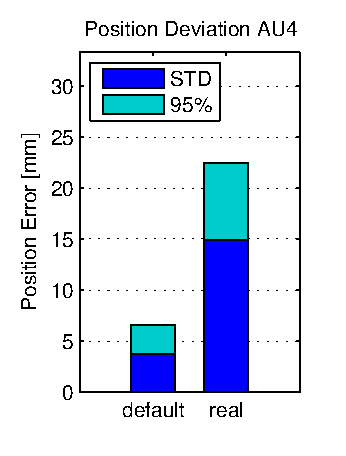
\includegraphics[width=0.24\textwidth]{images/results/err_cmp_real_pos.eps}
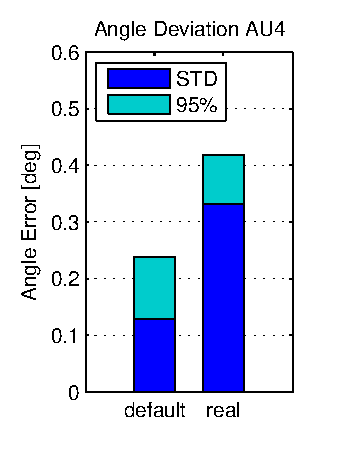
\includegraphics[width=0.24\textwidth]{images/results/err_cmp_real_angle.eps} %\\
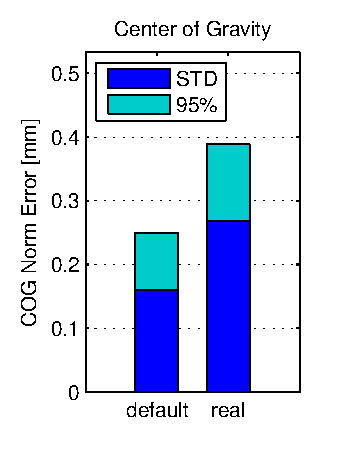
\includegraphics[width=0.24\textwidth]{images/results/err_cmp_real_cog.eps}
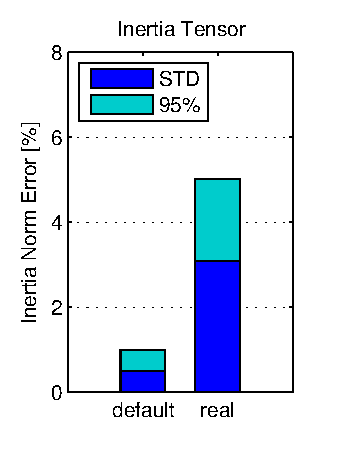
\includegraphics[width=0.24\textwidth]{images/results/err_cmp_real_tensor.eps}
\caption{Results for real system}
\label{fig:err_cmp_real}
\end{figure}

\subsection{Simulation Improvement}
By feeding the same actuator inputs of one of the real datasets to the simulation it should be possible to accurately reproduce the same dataset.
We can show that the default Skye model which has been used in the simulation of section~\ref{sub:est_perf} can be improved by using the results from the simulation to create the blimp mode.
This is because the default Skye model is based on CAD data and the real blimp deviates from the CAD data due to manufacturing tolerances.\\
The errors inside the green shaded areas of figure~\ref{fig:result_sim_improve_and_error} have been improved by roughly a factor of two.

\begin{figure}[hbtp]
\centering
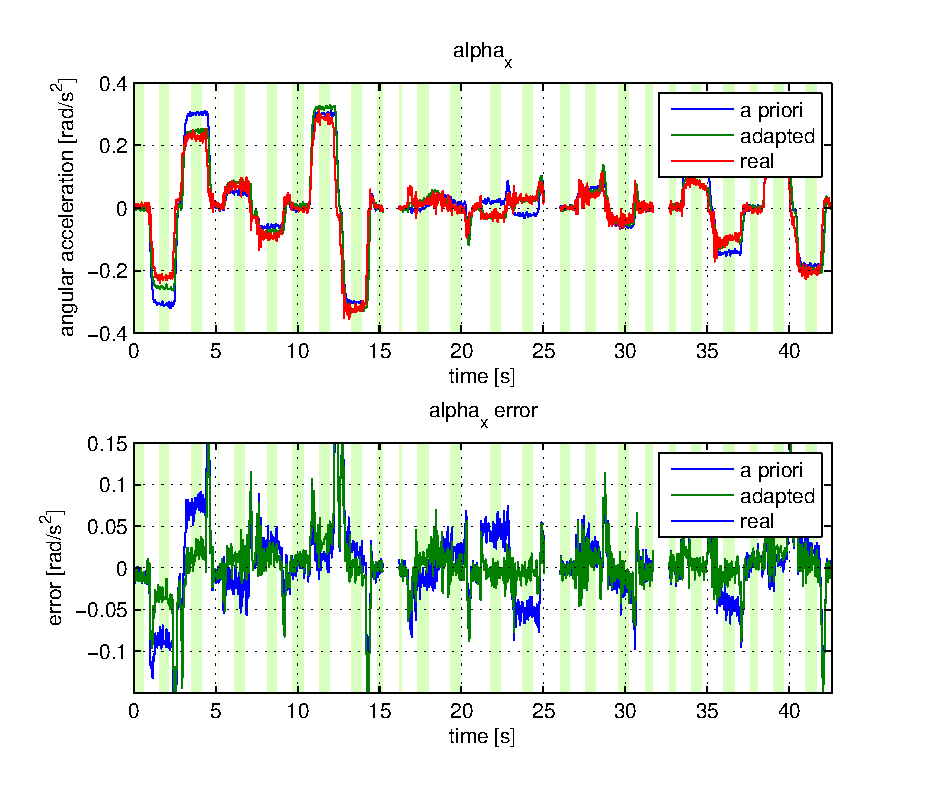
\includegraphics[scale=0.8]{images/results/compare_alpha_x.eps}
\caption{\textbf{Top}: \textbf{Red} is a section of alpha from the real system. \textbf{Blue} is the same section recreated by simulation with the default Skye simulation model. \textbf{Green} is the same section recreated by simulation with an Skye model which was adapted with the structure result from our batch optimisation. \textbf{Bottom}: The error of the recreated angular accelerations. We can see that the adapted simulation produces much better results. The error is high during input transients (the \textbf{white} areas of the plot). !!besser formuliere!!}
\label{fig:result_sim_improve_and_error}
\end{figure}

\section{Ground Truth}
...Do not tell toooo much in this section. Nobody likes to read long reports. So just mention 'we did it' and show the results.

...